\documentclass{article}

\usepackage{amsmath}    % Math formatting
\usepackage{amsfonts}   % Math formatting
\usepackage{amssymb}    % Math formatting
%\usepackage{fullpage}   % Use full page
\usepackage{setspace}   % Allow double spacing
\usepackage{graphicx}   % Include images
\usepackage{times}      % Use Times New Roman font
\usepackage{pdfpages}   % Include pdfs
\usepackage{tikz}       % Create Pictures
\usepackage{pgfplots}   % Create Pictures
\usepackage{caption}    % Figure captioning
\usepackage{subcaption} % Figure captioning
\usepackage{hyperref}   % movie dependence
\usepackage{movie15}    % include animated .gifs
\usepackage{attachfile} % AttachFiles

\RequirePackage[l2tabu, orthodox]{nag} % Nag about bad syntax


\newcommand{\nvec}[1]{\left\langle #1 \right\rangle}
\newcommand{\abs}[1]{\left\lvert #1 \right\rvert}

\begin{document}

\title{\attachfile{CalcIIINotes.tex}{Calc III Notes (APPM 2350)}}
\author{Zoe Farmer}
\maketitle

\tableofcontents
\addcontentsline{toc}{section}{Calculus III Contents}
\listoffigures
\addcontentsline{lof}{section}{Calculus III Figures}

\begin{figure}[h]
    \centering
    \includegraphics[scale=0.25]{break.png}
\end{figure}

In this course we will primarily interact with three dimensional space, therefore it is critical to thoroughly understand three dimensions. After three dimensional space we will move on to calculus in three dimensions and associated functions.

\section{Three Dimensional Space}
We call 2-dimensional space $ \mathbb{R}^2 $, therefore 3-dimensional space is represented by $ \mathbb{R}^3 $.

    \subsection{Circles and Spheres}
    In $\mathbb{R}^2$ we use the formula $(x-x_0)^2+(y-y_0)^2=r^2$ for circles. In $\mathbb{R}^3$ we add the $z$ factor to get
    \begin{equation}
    (x-x_0)^2+(y-y_0)^2+(z-z_0)^2=r^2
    \end{equation}

    \subsection{Distance Formula}1
    Distance between two points can be defined as

    \begin{equation}
    d((x, y, z), (x_0, y_0, z_0)) = \sqrt{(x - x_0)^2 + (y - y_0)^2 + (z - z_0)^2}
    \end{equation}

\section{Vectors}
A vector possesses both magnitude as well as direction. However the magnitude and direction are the only important parts of a vectors. In other words, the position of the vector is arbitrary, moving the vector around doesn't change the vector itself.

    \subsection{Scalar Multiples of Vectors}
    These multiples extend the vectors as well as possible switch the direction.
    \begin{equation}
        c \cdot \vec{v} = \begin{cases}
            c > 0, \text{Extends in the same direction}\\
            c < 0, \text{Flips 180 and extends}
        \end{cases}
    \end{equation}

    \subsection{Addition and Subtraction of Vectors}
    Two methods can be used, tip to tail or parallelogram (see picture for graphical representation).
    Algebraically this operation can be completed by combining the components of the vectors:\\
    $\vec{v_1}+\vec{v_2}=(x_1+x_2)\hat{\imath}+(y_1+y_2)\hat{\jmath}+(z_1+z_2)\hat{k}$
    \begin{figure}[ht]
        \centering
        \includegraphics[scale=.5]{vectorparallelogram.png}
        \caption{Vector Parallelogram}
    \end{figure}

    \subsection{Vector Properties}
        \subsubsection{Magnitude}
        The magnitudes of vectors an be found using: $|\vec{v}|=\sqrt{x^2+y^2+z^2}$
        \subsubsection{Scalar Multiplication}
        $\text{let }c\neq 0\text{ and } \vec{v}=x\hat{\imath}+y\hat{\jmath}+z\hat{k}\\c\vec{v}=(cx)\hat{\imath}+(cy)\hat{\jmath}+(cz)\hat{k}\\|c\vec{v}|=|c||\vec{v}|$

    \subsection{Inner Product (Dot Product)}
    This is the first method of vector multiplication.\\
    If $\vec{A} \cdot \vec{B} = 0$, then the two vectors are orthogonal.\\
    Formula = $\vec{A} \cdot \vec{B} = |\vec{A}||\vec{B}|\cos(\theta)$\\
    You can also use the law of cosines:
    $\vec{A} \cdot \vec{B} = \frac{1}{2}(|\vec{A}|^2+|\vec{B}|^2-|\vec{B}-\vec{A}|^2)$\\
    Or $\vec{A} \cdot \vec{B} = A_1B_1+A_2B_2+A_3B_3$

        \subsubsection{Rules of Dot Products}
        $\vec{A} \cdot \vec{B} = \vec{B} \cdot \vec{A}$\\
        $|\vec{A}|^2 = \vec{A} \cdot \vec{A}$\\
        $c(\vec{A} \cdot \vec{B}) = (c\vec{A}) \cdot \vec{B} = \vec{A} \cdot (c\vec{B})$\\
        $\vec{A} \cdot (\vec{B} + \vec{C}) = \vec{A} \cdot \vec{B} + \vec{A} \cdot \vec{C}$

        \subsubsection{Example - Dot Product}
        \[
        \begin{aligned}
        \begin{tabular}{l | l}
        $\vec{A} = \langle 1,0,2 \rangle$ & Given\\
        $\vec{B} = \langle 2,0,1 \rangle$ & Given\\
        $\vec{A} \cdot \vec{B} = (1 \cdot 2) + (0 \cdot 0) + (2 \cdot 1) = 4$ & $\vec{A} \cdot \vec{B} = A_1B_1+A_2B_2+A_3B_3$\\
        $|\vec{A}| = \sqrt{2^2 + 0^2 + 1^2} = \sqrt{5}$ & $|\vec{v}|=\sqrt{x^2+y^2+z^2}$\\
        $|\vec{B}| = \sqrt{1^2 + 0^2 + 2^2} = \sqrt{5}$ & $|\vec{v}|=\sqrt{x^2+y^2+z^2}$\\
        $4 = \sqrt{5}^2 \cos(\theta)$ & $\vec{A} \cdot \vec{B} = |\vec{A}||\vec{B}|\cos(\theta)$\\
        $\cos(\theta) = \frac{4}{5}$ & Solve for $\theta$\\
        $\theta = \arccos(\frac{4}{5})$ & \\
        \end{tabular}
        \end{aligned}
        \]

    \subsection{Projections}
    Formula for projections: $Proj_{\vec{A}}\vec{B}=|\vec{B}|\cos(\theta)\frac{\vec{A}}{|\vec{A}|}$
    \begin{figure}[ht]
        \centering
        \includegraphics[scale=.5]{projection.JPG}
        \caption{$\vec{u}=\vec{a} \text{ and } \vec{v}=\vec{b}$}
    \end{figure}

        \subsubsection{Example - Projection}
        \[
        \begin{aligned}
        \text{Find }Proj_{\vec{A}} \vec{B}\\
        \vec{B} = \nvec{6,3,2}\\
        \vec{A} = \nvec{1,-2,-2}\\
        \frac{\vec{A} \cdot \vec{B}}{{|\vec{A}|^2}}\\
        \vec{A} \cdot \vec{B} = -4\\
        |\vec{A}|^2 = 1^2 + (-2)^2 + (-2)^2 = 9\\
        Proj_{\vec{A}} \vec{B} = \frac{-4}{9} \cdot \nvec{1,-2,-2}\\
        \end{aligned}
        \]

    \subsection{Vector Cross Products}
    This is the second method of vector multiplication.\\
    \begin{equation}
    \begin{aligned}
    |\vec{A}\times\vec{B}=|\vec{A}||\vec{B}|\sin(\theta)\\
    \vec{A}\times\vec{B}=\langle (A_2B_3-A_3B_2),-(A_1B_3-A_3B_1),(A_1B_2-A_2B_1) \rangle\\
    \begin{vmatrix}
    \hat{\imath} & \hat{\jmath} & \hat{k}\\
    A_1 & A_2 & A_3\\
    B_1 & B_2 & B_3\\
    \end{vmatrix}
    = \begin{vmatrix}
    A_2 & A_3\\
    B_2 & B_3\\
    \end{vmatrix} \hat{\imath}-
    \begin{vmatrix}
    A_1 & A_3\\
    B_1 & B_3\\
    \end{vmatrix} \hat{\jmath}+
    \begin{vmatrix}
    A_1 & A_2\\
    B_1 & B_2\\
    \end{vmatrix} \hat{k}
    \end{aligned}
    \end{equation}

        \subsubsection{Rules of Cross Products}
        $\vec{A}\times(\vec{B}+\vec{C})=\vec{A}\times\vec{B}+\vec{A}\times\vec{C}$\\
        $|\vec{A}\times\vec{B}|=$Area of parallelogram\\
        Volume of a parallelpipen:
        \begin{equation}
        |\vec{A}\cdot(\vec{B}\times\vec{C})|=
        \begin{vmatrix}
        A_1 & A_2 & A_3\\
        B_1 & B_2 & B_3\\
        C_1 & C_2 & C_3\\
        \end{vmatrix}
        \end{equation}
        \subsubsection{Example - Cross Product}
        \[
        \begin{aligned}
        \vec{A}=\nvec{2,1,1};\vec{B}=\nvec{-4,3,1}\\
        \begin{vmatrix}
        \hat{\imath} & \hat{\jmath} & \hat{k}\\
        2 & 1 & 1 \\
        -4 & 3 & 1\\
        \end{vmatrix}\\
        (1-3)\hat{\imath}-(2+4)\hat{\jmath}+(6+4)\hat{k}\\
        -2\hat{\imath}-6\hat{\jmath}+10\hat{k}\\
        \end{aligned}
        \]

\section{Lines and Planes}

    We can find the formula for a line in three dimensional space.\\

    \subsection{Lines}
    Building a line in $\mathbb{R}^3$:
    \begin{enumerate}
    \item Find a point $(x_0,y_0,z_0)$
    \item Find a vector $\vec{v}=(v_1,v_2,v_3)$
    \item Vector between $(x(t),y(t),z(t))$ and $(x_0,y_0,z_0)$ is $\langle x(t)-x_0,y(t)-y_0,z(t)-z_0\rangle = t\nvec{v_1,v_2,v_3}$
    \item \begin{equation}
    \boxed{\text{Equation of a Line:}\\
        \begin{cases}
            x(t)=x_0+tv_1\\
            y(t)=y_0+tv_2\\
            z(t)=z_0+tv_3
        \end{cases}}
    \end{equation}
    \end{enumerate}

        \subsubsection{Example - Building a Line in $\mathbb{R}^3$}
        Given point $P_0(-2,0,4)$ and vector $\vec{v}=\nvec{2,4,-2}$\\
        \[
            \begin{cases}
                x(t)=-2+2t\\
                y(t)=0+4t\\
                z(t)=4-2t
            \end{cases}
        \]

        \subsubsection{Example - Building a Line in $\mathbb{R}^3$}
        Find an equation for the line between $P(-3,2,-3)$ and the point $Q(1,-1,4)$\\
        \[
        \begin{aligned}
            \vec{PQ}=\nvec{4,-3,7}\\
            \begin{cases}
                x(t)=-3+4t\\
                y(t)=2-3t\\
                z(t)=-3-7t
            \end{cases}
        \end{aligned}
        \]

        \subsubsection{Example - Distance from a Point to a Line}
        Distance from a point $s$ to a line $l$
        \[
        \begin{aligned}
        d=|\vec{PS}|\sin(\theta)\\
        |\vec{PS}\times\vec{v}|=|\vec{PS}||\vec{v}|\sin(\theta)\\
        |\vec{PS}|\sin(\theta)=\frac{|\vec{SP}\times\vec{v}|}{|\vec{v}|}\\
        \text{Distance from }s\text{ to }l\equiv d=\frac{|\vec{SP}\times\vec{v}|}{|\vec{v}|}
        \end{aligned}
        \]

    \subsection{Planes}

    We can also find the formula for a plane in three dimensional space.\\

    Equation for a plane
    \begin{enumerate}
    \item Point $P_0=(x_0,y_0,z_0)$ on the plane
    \item Need to find the normal vector $\vec{n}=\nvec{A,B,C}$ where $\vec{n}\bot\vec{P_0P}$
    \end{enumerate}
    Formula for a plane: $\vec{r}(t)=P_0+vt\equiv\vec{r}(t)=(x_0,y_0,z_0)+\nvec{A,B,C}t$

        \subsubsection{Example - Find a Point on the Plane}
        Given $2x+3y+9z=\pi$ and $\vec{n}=\nvec{2,3,9}$, find a point on the plane.
        \[
        \begin{aligned}
        \text{let }x=y=0\\
        \therefore z=\frac{\pi}{9}\\
        P_0=(0,0,\frac{\pi}{9})\\
        \end{aligned}
        \]

        \subsubsection{Example - Building a Plane in $\mathbb{R}^3$}
        Find the equation for the place through points $P=(0,0,1),Q=(2,0,0),R=(0,3,0)$
        \[
        \begin{aligned}
        \vec{PQ}=\nvec{2,0,-1}\\
        \vec{PR}=\nvec{0,3,-1}\\
        \vec{PQ}\times\vec{PR}=
            \begin{vmatrix}
                \hat{\imath} & \hat{\jmath} & \hat{k}\\
                2 & 0 & -1 \\
                0 & 3 & -1 \\
            \end{vmatrix}
        =3\hat{\imath} + 2\hat{\jmath} + 6\hat{k}\\
        3x+2y+6z=6
        \end{aligned}
        \]


\section{Assorted Quadric Surfaces}
    There are several shapes that are necessary for much of this course. Memorize these\dots

    \begin{figure}[h!]
        \includegraphics[scale=0.4]{quadricsurfaces.png}
        \caption{Table of Quadric Surfaces}
    \end{figure}

\newpage

\section{Vector Functions}
Input of a single value ($t,t\in\mathbb{R}$) like a parametric function.\\
$\vec{r}(t)=$vector$\in [\mathbb{R}^2,\mathbb{R}^3]\\
\vec{r}(t)=x(t)\hat{\imath} + y(t)\hat{\jmath} + z(t)\hat{k}\\
\vec{r}(t)=\nvec{x(t),y(t),z(t)}$
\subsubsection{Example - Lines}
$
\vec{r}(t)=P_0+vt\\
\vec{r}(t)=\nvec{x_0+at,y_0+bt,z_0+ct}
$

    \subsection{Intersections of Surfaces}
    Given $z=y^2+1$ and $x^2+\frac{y^2}{4}=1$\\
    $
    \therefore x(t)=\cos(t)\\
    y(t)=2\sin(t)\\
    z(t)=4\sin^2(t)+1\\
    \nvec{\cos(t),2\sin(t),4\sin^2(t)+1}\\
    $

\section{Calculus of Vector Functions}
\begin{enumerate}
\item Limits - These can be taken with respect to each component, one at a time.
\item Derivatives - These can be taken with respect to each component, one at a time.
\item Integrals
\end{enumerate}

\section{Tangent Vectors}
Definition: Unit Tangent vector $\hat{T}(t) = \frac{\vec{r}\prime(t)}{|\vec{r}\prime(t)|}$\\
$ \vec{r}\prime(t)$ points in the direction of trajectory.

\section{Arc Length}
Arc length of any given path $\vec{r}(t)$ can be calculated.
\begin{equation}
\text{Arc length }s\text{ between }r(t_0)\text{ and }r(t_f) \equiv \int_{t_0}^{t_f} |\vec{v}(t)|dt = \int_{t_0}^{t_f} |\vec{r}\prime(t)|dt
\end{equation}
Arc length is important because it allows us to calculate vectors around a given line in $\mathbb{R}^3$.\\

Another important concept is the Arc Length Parameter $s(t)$.

\begin{equation}
s(t) = \int_{t_0}^{t} |\vec{v}(t)|dt
\end{equation}

\section{The TNB Frame}
\begin{figure}[h]
\centering
    \includegraphics[scale=1]{tnb.png}
    \caption{The TNB Frame}
\end{figure}

The TNB frame is at its core a method for describing a line in 3 dimensional space. At any given point the line in question will have a Tangent vector, a Normal vector, and a Binormal vector. Note, all three of these vectors are orthagonal to each other.\\

The Tangent Vector describes the direction of motion in space as well as the velocity of a particle at that point.
\begin{equation}
\hat{T} = \frac{\frac{d\vec{r}}{dt}}{\abs{\frac{d\vec{r}}{dt}}} =
\frac{\vec{r}\prime(t)}{\abs{\vec{r}\prime(t)}}
\end{equation}

The Normal Vector describes the tendency for the line to curve in space as well as centripetal acceleration.
\begin{equation}
\hat{N} = \frac{\frac{d\hat{T}}{ds}}{\abs{\frac{d\hat{T}}{ds}}}
\end{equation}

The Binormal Vector describes the tendency for the line to leave the plane.
\begin{equation}
\hat{B} = \hat{T} \times \hat{N}
\end{equation}

These three components also give us curvature
\begin{equation}
\kappa = \abs{\frac{d\hat{T}}{ds}} = \frac{\abs{\vec{v}\times\vec{a}}}{\abs{\vec{v}}^3}
\end{equation}
\indent And torsion
\begin{equation}
\tau = \frac{
    \begin{vmatrix}
    \dot{x} & \dot{y} & \dot{z}\\
    \ddot{x} & \ddot{y} & \ddot{z}\\
    \dddot{x} & \dddot{y} & \dddot{z}\\
    \end{vmatrix}
}{\abs{\vec{v}\times\vec{a}}^2}
\end{equation}

\section{Partial Derivatives}
In order to find the derivative at any given point on a 3 dimensional surface, you need to essentially ``fix'' one variable and treat it as a constant. This allows you to look at a line as opposed to a surface.

\begin{figure}[h]
\centering
    \includegraphics[scale=0.5]{partials.png}
    \caption{Cross Sections of a Partial Derivative}
\end{figure}

Some notation:

\[
\frac{\partial f}{\partial x} = \partial_xf \text{ and }
\frac{\partial f}{\partial y} = \partial_yf
\]

Double and triple partials are also allowed, and for most instances
\[
\partial_{xy} = \partial_{yx}
\]

    \subsection{Example - $ f(x, y) = x^2 + 3xy + y - 1 $}
    \[
    \begin{aligned}
    \begin{cases}
    \partial_x = 2x + 3y \to \text{($y$ acts as a constant)}\\
    \partial_y = 3x + 1 \to \text{($x$ acts as a constant)}
    \end{cases}
    \end{aligned}
    \]

\section{Tangent Planes}
At any point on a given surface there exists a plane tangent to the point.
\begin{figure}
\centering
    \includegraphics[scale=0.75]{tplane.png}
    \caption{Tangent Plane with Associated Normal}
\end{figure}
The equation for this tangent plane is as follows
\begin{equation}
\begin{aligned}
f_x(x_0, y_0)(x - x_0) + f_y(x_0, y_0)(y - y_0) - (z - f(x_0, y_0)) = 0\\
\text{ where } f_x = \frac{\partial f}{\partial x} \text{ and } f_y = \frac{\partial f}{\partial y}
\end{aligned}
\end{equation}
The normal vector to this tangent plane is
\begin{equation}
\nabla f(x_0, y_0, z_0)
\end{equation}
\section{Linear Approximation}
This is to approximate the value of the surface function at any given point by using a plane tangent to the surface at that point. Therefore this formula is a variation on the tangent plane formula.
\begin{equation}
\mathcal{L}_{f(x_0, y_0)}(x, y) = f(x_0, y_0) + f_x(x_0, y_0)(x - x_0) + f_y(x_0, y_0)(y - y_0)
\end{equation}
    \subsection{Example - Find the approximate value of $f(x, y) = 2x^2 + y^2$ at the point $(1.1,1.1)$.}
    \[
    \begin{aligned}
    \mathcal{L}_{f(x_0, y_0)}(x, y) &= f(x_0, y_0) + f_x(x_0, y_0)(x - x_0) + f_y(x_0, y_0)(y - y_0)\\
    \mathcal{L}_{f(1.1, 1.1)}(x, y) &= 3 + 4(1.1-1) + 2(1.1-1) \approx 3.6
    \end{aligned}
    \]
\section{Differential}
\begin{equation}
\begin{aligned}
dx = \Delta x = x - x_0\\
dy = \Delta y = y - y_0\\
dz = \Delta z = z - z_0\\
\end{aligned}
\end{equation}
    \subsection{Relative Error}
    \begin{equation}
    \begin{aligned}
    \text{Error}
    \begin{cases}
    \frac{dx}{x}\\
    \frac{dy}{y}\\
    \frac{dz}{z}
    \end{cases}
    \end{aligned}
    \end{equation}
\section{Chain Rule}
Let $ z = f(x, y) $ where $x$ and $y$ are functions in terms of $t \to x(t),y(t)$. Therefore we can define $z$ in terms of $t \to z(t)=f(x(t), y(t))$. Given this, we can find the derivative of $z$ in terms of $t$.
\begin{equation}
\frac{dz}{dt} = \frac{\partial z}{\partial x} \frac{dx}{dt} + \frac{\partial z}{\partial y} \frac{dy}{dt}
\end{equation}
If $x$ and $y$ are in terms of $t$ and $s$, then we can do two different chain rules.
\begin{equation}
\begin{aligned}
\frac{dz}{dt} = \frac{\partial z}{\partial x} \frac{dx}{dt} + \frac{\partial z}{\partial y} \frac{dy}{dt}\\
\frac{dz}{ds} = \frac{\partial z}{\partial x} \frac{dx}{ds} + \frac{\partial z}{\partial y} \frac{dy}{ds}
\end{aligned}
\end{equation}
\section{Directional Derivative}
If we wish to know how $f$ changes in terms of $x$ or $y$, we can find the derivative. However if we instead wish to know how $f$ changes in a given direction $\vec{u} = \nvec{u_1, u_2}$ we use
\begin{equation}
D_{\vec{u}}f = \nvec{\frac{df}{dx}, \frac{df}{dy}} \cdot \nvec{u_1, u_2} = \nabla f \cdot \vec{u}
\end{equation}
Where we define the gradient of a function $f$
\begin{equation}
\nabla f = \nvec{f_x, f_y}
\end{equation}
\section{Level Curves}
Level curves are the two dimensional projection of a surface on the $xy$ plane. Think of a contour map, the closer together the curves are, the steeper the slope of the surface is.
\begin{figure}[h]
\centering
    \includegraphics[scale=0.5]{levelcurve.png}
    \caption{A Surface and its Associated Level Curves}
\end{figure}
With any given level curve, the gradient of the surface will always be orthogonal to the level curves.
\begin{figure}[h]
\centering
    \includegraphics[scale=0.5]{levelgrad.png}
    \caption{Gradient of a Level Curve}
\end{figure}
\section{Extrema}
In order to find local minima and maxima, we need to find points at which $f_x(x,y)=0,f_y(x,y)=0, \text{ and }\nabla f=0$. The $(x,y)$ coordinates that satisfy these equations are called critical points. In other words, solve the gradient for zero. Once critical points have been identified, there are a couple tests to do to identify the types for each critical point.\\

First compute the Hessian
\begin{equation}
\det \left(
\begin{vmatrix}
f_{xx} & f_{xy}\\
f_{xy} & f_{yy}
\end{vmatrix} \right) =
f_{xx} \cdot f_{yy} - f_{xy}^2
\end{equation}
Then there are three different situations
\begin{equation}
\begin{aligned}
\begin{cases}
\text{Hessian} > 0 \to
    \begin{cases}
    [f_{xx}\text{ or }f_{yy}] > 0 \to \text{Minimum}\\
    [f_{xx}\text{ or }f_{yy}] < 0 \to \text{Maximum}
    \end{cases}\\
\text{Hessian} < 0 \to \text{Saddle}\\
\text{Hessian} = 0 \to \text{No Conclusions}
\end{cases}
\end{aligned}
\end{equation}
\section{Lagrangian Multipliers}
Essentially constrained optimization. Given a constraint $g(x, y)$, we can find maximum and minimum values of a function $f(x,y)$ on the constraint.\\

To find the maximums and minimums of $f$ on $g$, compute the langrangian multiplier $\lambda$ using $\nabla f = \lambda \nabla g$ and $g(x,y)=c$.

    \subsection{Example - Find the points on $x^2 - z^2 - 1 = 0$ that are closest to the origin.}
    \begin{equation}
    \begin{aligned}
    g = x^2 - z^2 - 1 = 0\\
    f = x^2 + y^2 + z^2\\
    \nabla g = \nvec{2x, 0, -2z}\\
    \nabla f = \nvec{2x, 2y, 2z}\\
    \nvec{2x, 2y, 2z} = \lambda \nvec{2x, 0, -2z}\\
    \text{Solve the system of equations}\\
    x \pm 1, y = 0, z = 0, \lambda = 1\\
    \text{Therefore our critical points are at } (1,0,0) \text{ and } (-1,0,0)
    \end{aligned}
    \end{equation}
\section{Double Integrals}
We can find area and volume of given shapes using double integrals. In order to find the integral, you first take it with respect to one axis, and then the other. The order of integration is irrelevant.\\
\begin{equation}
\text{Fabini's Theorem: } \iint\limits_R f(x,y)dA \to \int_a^b \left( \int\limits_c^d f(x,y)dy\right) dx \equiv \int\limits_c^d \left( \int_a^b f(x,y)dx\right) dy
\end{equation}
The hardest part of multiple integration is determining the bounds of integration. The integral itself is usually not too tricky, however the bounds often pose an issue.
    \subsection{Example - Switch the order of integration for the given integrals}
    \[
    \begin{aligned}
    \text{Given } \int_0^1 \int_{\sqrt{y}}^1 f(x,y) dxdy\\
    \text{Bounds}\begin{cases}
    \sqrt{y} \le x \le 1\\
    0 \le y \le x^2
    \end{cases}\\
    \int_0^1 \int_0^{x^2} f(x,y) dydx
    \end{aligned}
    \]
    \begin{figure}[ht]
    \centering
        \includegraphics[scale=0.25]{example.png}
    \caption{The Given Bounds}
    \end{figure}

\section{Double Integrals in Polar Coordinates}
In Cartesian Coordinates you either use vertical or horizontal slices to determine the overall area. With Polar Coordinates you instead either use a sets of wedges or expanding washers.
\[
\iint\limits_R f(x,y)dA = \iint\limits_R f(r, \theta) dA = \iint\limits_R f(r, \theta) rdrd\theta
\]
    \subsection{Example - Find the area of the lemniscate $r^2 = 4\cos(2\theta)$.}
    \[
    \int_0^{\frac{\pi}{4}} \int_0^{2 \sqrt{\cos(2\theta)}} rdrd\theta = 1
    \]
\section{Triple Integrals}
Triple integrals calculate the volume of a specified region. To determine bounds, approach from one direction and then integrate over the identified region.
    \subsection{Example - Find the Volume in Six Ways}
    Given: $R$ is a tetrahedron with vertices at $[(0,0,0), (1,1,0), (0,1,0), (0,1,1)]$.
    \[
    \begin{aligned}
    \text{Normal of the plane defining the region} = \nvec{-1,1,-1} \therefore z=y-x\\
    \int_0^1 \int_x^1 \int_0^{y-x} F(x,y,z) dzdydx\\
    \int_0^1 \int_0^y \int_0^{y-x} F(x,y,z) dzdxdy\\
    \int_0^1 \int_z^1 \int_0^{y-z} F(x,y,z) dxdydz\\
    \int_0^1 \int_0^y \int_0^{y-z} F(x,y,z) dxdzdy\\
    \int_0^1 \int_0^{1-x} \int_{z+x}^1 F(x,y,z) dydzdx\\
    \int_0^1 \int_0^{1-z} \int_{z+x}^1 F(x,y,z) dydxdz\\
    \end{aligned}
    \]
\section{Cylindrical and Spherical Coordinates}
Cartesion is all about grids, Cylindrical is stacked polar graphs, and Spherical is a series of layered spheres as the name implies. For cylindrical, it is essentially just polar with an extra dimension. Any point in the plane can be described as a point on the circle with radius $r$.\\
Note, radius can never be negative.

    \subsection{Conversion from Cartesion to Cylindrical}
    $
    \begin{aligned}
    x=r\cos(\theta)\\y=r\sin(\theta)\\z=z
    \end{aligned}
    $

    \begin{figure}[ht]
    \centering
        \begin{tikzpicture}
        \draw[->] (-0.2,0) -- (2.2,0) node[right] {$r$};
        \draw[->] (0,-0.2) -- (0,2.2) node[right] {$z$};
        \draw[->] (0,0) -- (2,2) node[right] {$r=z$};
    \end{tikzpicture}
    \caption{The $rz$ plane}
    \end{figure}

    \subsection{Conversion from Cartesion to Sperical Coordinates}
    $
    \begin{aligned}
    x=\rho \sin(\phi)\cos(\theta)\\
    y=\rho \sin(\phi)\sin(\theta)\\
    z=\rho \cos(\phi)
    \end{aligned}
    $

    \begin{figure}[ht]
    \centering
        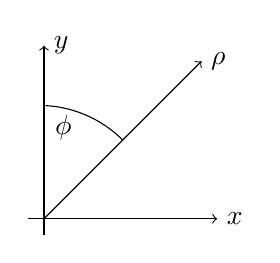
\begin{tikzpicture}
        \draw[->] (-0.2,0) -- (2.2,0) node[right] {$x$};
        \draw[->] (0,-0.2) -- (0,2.2) node[right] {$y$};
        \draw[->] (0,0) -- (2,2) node[right] {$\rho$};
        \draw (1,1) arc(45:87:1.5cm) node[below right] {$\phi$};
        \end{tikzpicture}
    \caption{The $\rho \phi$ plane}
    \end{figure}

    \subsection{Example - Describe the region between $x^2 + y^2 + z^2 = 4$ and $z=\sqrt{x^2 + y^2}$.}

    \[
    \begin{aligned}
    \text{Convert Coordinates}\\
    x^2 + y^2 = 4-z^2\\
    \rho^2 \sin^2(\phi)\cos^2(\theta) + \rho^2 \sin^2(\phi) \sin^2(\theta) = 4 - \rho^2 \cos^2(\phi)\\
    \rho^2 \sin^2(\phi) = 4 - \rho^2 \cos^2(\phi)\\
    \rho^2(\sin^2(\phi) + \cos^2(\phi)) = 4\\
    \rho^2 = 4\\
    \rho = 2
    \end{aligned}
    \leftrightarrows
    \begin{aligned}
    z = \sqrt{x^2 + y^2}\\
    \phi = \frac{\pi}{4}
    \end{aligned}
    \]

    \begin{figure}[ht]
    \centering
        \begin{subfigure}[b]{0.3\textwidth}
            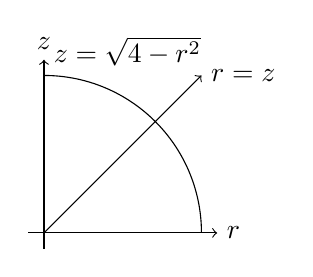
\begin{tikzpicture}
                \draw[->] (-0.2,0) -- (2.2,0) node[right] {$r$};
                \draw[->] (0,-0.2) -- (0,2.2) node[above] {$z$};
                \draw[->] (0,0) -- (2,2) node[right] {$r=z$};
                \draw (2,0) arc(0:90:2cm) node[above right] {$z=\sqrt{4-r^2}$};
            \end{tikzpicture}
            \caption{The region in the $rz$ plane}
            \label{fig:sub1}
        \end{subfigure}
        \begin{subfigure}[b]{0.3\textwidth}
            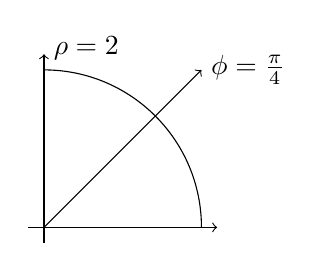
\begin{tikzpicture}
                \draw[->] (-0.2,0) -- (2.2,0);
                \draw[->] (0,-0.2) -- (0,2.2);
                \draw[->] (0,0) -- (2,2) node[right] {$\phi=\frac{\pi}{4}$};
                \draw (2,0) arc(0:90:2cm) node[above right] {$\rho = 2$};
            \end{tikzpicture}
            \caption{The region in the $\rho \phi$ plane}
            \label{fig:sub1}
        \end{subfigure}
        \caption{The example in various coordinate systems}
    \end{figure}

    \[
        \begin{aligned}
        \text{Cylindrical Coordinate Region: }& \begin{cases}
            0 \le r \le \sqrt{2}\\
            r \le z \le \sqrt{4-r^2}
        \end{cases}\\
        \text{Spherical Coordinate Region: }& \begin{cases}
            0 \le \rho \le 2\\
            0 \le \phi \le \frac{\pi}{4}
        \end{cases}
        \end{aligned}
    \]


    \subsection{Jacobians for Cartesion, Cylindrical, and Spherical Coordinates}
    \begin{equation}
    \begin{aligned}
    \text{Cartesion: }& dV=dxdydz\\
    \text{Cylindrical: }& dV=rdrdzd\theta\\
    \text{Spherical: }& dV=\rho^2 \sin(\phi) dpd\phi d\theta\\
    \end{aligned}
    \end{equation}

\section{Change of Variables}
Let's assume that we have some function $f(x,y)$, and both $x$ and $y$ can be defined as functions wih respect to $u$ and $v$. In other words:
\[
\begin{aligned}
\begin{cases}
x = x(u,v) \to \text{ e.g. } x \equiv x(r, \theta) = r \cos(\theta) \\
y = y(u,v) \to \text{ e.g. } y \equiv y(r, \theta) = r \sin(\theta)
\end{cases}\\\\\\
\text{We essentially wish to do this: }
\iint f(x,y) dxdy \to \iint f(u,v) \frac{dxdy}{dudv}dudv\\\\
\text{ We use } \frac{dxdy}{dudv} = \frac{\partial (x,y)}{\partial (u,v)} \text{ which we call the Jacobian } J(u,v)\\
\end{aligned}
\]

    \subsection{Formal Definition of Jacobian}
    \begin{equation}
    \begin{aligned}
        J(u,v) = \frac{\partial (x,y)}{\partial (u,v)} = 
        \left\lvert
        \det
        \begin{vmatrix}
        \frac{\partial x}{\partial u} & \frac{\partial x}{\partial v}\\
        \frac{\partial y}{\partial u} & \frac{\partial y}{\partial v}\\
        \end{vmatrix}\right\rvert = 
        \left\lvert
        \det
        \begin{vmatrix}
        X_u & X_v \\
        Y_u & Y_v \\
        \end{vmatrix}
        \right\rvert = 
        \left\lvert
        \frac{\partial x}{\partial u}\cdot\frac{\partial y}{\partial v} - \frac{\partial x}{\partial v}\cdot\frac{\partial y}{\partial u}
        \right\rvert
    \end{aligned}
    \end{equation}
    $\therefore dA = dxdy = J(u,v)dudv$

    \subsection{Example for Polar Coordinates - What's the Jacobian if $x=r\cos(\theta)$ and $y=r\sin(\theta)$?}
    \[
    \begin{aligned}
        J(u,v) = \frac{\partial (x,y)}{\partial (u,v)} = 
        \left\lvert
        \det
        \begin{vmatrix}
        \frac{\partial x}{\partial u} & \frac{\partial x}{\partial v}\\
        \frac{\partial y}{\partial u} & \frac{\partial y}{\partial v}\\
        \end{vmatrix}\right\rvert = 
        \left\lvert
        \det
        \begin{vmatrix}
        \cos(\theta) & -r\sin(\theta) \\
        \sin(\theta) & -r\cos(\theta)
        \end{vmatrix}
        \right\rvert = 
        \left\lvert
        r\cos^2(\theta)+r\sin^2(\theta)
        \right\rvert = r\\
        \therefore dA=dxdy=rdrd\theta
    \end{aligned}
    \]

    \subsection{3 Dimensions}
    \begin{equation}
    \begin{aligned}
    J(u,v,w) = \frac{\partial (x,y,z)}{\partial (u,v,z)} = 
    \left\lvert
    \det
    \begin{vmatrix}
    X_u & X_v & X_w \\
    Y_u & Y_v & Y_w \\
    Z_u & Z_v & Z_w \\
    \end{vmatrix}
    \right\rvert
    \end{aligned}
    \end{equation}

\section{Application of Multiple Integrals}
We can use double and triple integrals to determine a number of different physical quantities.\\

To determine the mass of a plane with density $ \delta $

\begin{equation}
\text{Mass} = \iint\limits_R \delta (x,y) \, dA
\end{equation}\\

To find the Moment of the region around the $[x,y]$ axis

\begin{equation}
\text{Moment}_{[x,y]} = M_{[x,y]} = \iint\limits_R [x,y]\delta(x,y) \, dA
\end{equation}\\

Therefore we can calculate the coordinates of the center of mass of the region

\begin{equation}
\left( \bar{x} = \frac{M_x}{m} = \frac{\iint\limits_R x \delta(x,y) \, dA}{\iint\limits_R \delta (x,y) \, dA} \, , \,
\bar{y} = \frac{M_y}{m} = \frac{\iint\limits_R y \delta(x,y) \, dA}{\iint\limits_R \delta (x,y) \, dA} \right)
\end{equation}
\section{Vector Fields}
A vector field is a vector valued function. In other words, at any given point a vector value is given at that point.\\
\begin{figure}[ht]
\centering
    \includegraphics[scale=0.5]{3D-Vector-Field-chart.png}
\caption{3 Dimensional Vector Field}
\end{figure}
There are several different types of vector fields, but all are forces. One such field is a gravitational force field, another is an electrical force field. There are many such force fields including ones that deal with fluid mechanics.

There are two types of viewing vector field, the Lagrangian System where you look at the position of a particle at any given moment, and the Eulerian System where you look at the velocity of the particle at any given moment.

\section{Line Integrals}

Thus we can get the concept of a line integral. As any mass travels along a parametrized path in a vector field, work is done on that mass by the forces. $ w = \int\limits_c \vec{F} \cdot \hat{T} ds = \int\limits_c \vec{F} \cdot dr$

\begin{figure}
\centering
    \attachfile{lineint.gif}{Line Integral Animation}
\caption{Line Integral Animation}
\end{figure}

    \subsection{Example - Find $\int\limits_cf(x,y,z)ds$ with $f(x,y,z)=x-3y^2+z$ and the path defined as the line between points $(0,0,0)$ and $(1,1,1)$.}
    \[
    \begin{aligned}
    \text{First parametrize the line } \to \vec{r}(t)=\nvec{t,t,t}, 0 \le t \le 1\\
    \int\limits_c f(x,y,z)ds = \int_{t_0}^{t_f} f(x(t), y(t), z(t)) \frac{ds}{dt} dt\\
    = \int_{t_0}^{t_f} f(x(t), y(t), z(t)) |\vec{v}(t)| dt\\
    \text{\textit{If }} \vec{r}(t) = \nvec{t,t,t} \text{\textit{ Then }} \vec{v}(t) = \nvec{1,1,1}\\
    |\vec{v}|=\sqrt{3}\\
    t_0 = 0; t_f = 1\\
    \int_0^1(t-3t^2+t)\sqrt{3}dt = \sqrt{3}(t^2-t^3)\big{\vert}_0^1=0
    \end{aligned}
    \]

    \subsection{Flow}
    Circulation, or flow, can be described as the rate at which fluid is moving around the curve. Let's assume we have a vector field $\vec{u}$ and a curve defined by $\vec{r}(t)$.

    \begin{equation}
    \int\limits_c \vec{u} \cdot \hat{T} ds = \int\limits_c \vec{u} \cdot \frac{d\vec{r}}{ds} = \int\limits_c \vec{u} \cdot dr
    \end{equation}

    If we let $ \vec{u} = \nvec{M, N, P} $ and $ d\vec{r} = \nvec{dx, dy, dz} $, then we can define flow as:

    \begin{equation}
    Flow = \int\limits_c \nvec{M, N, P} \cdot \nvec{dx, dy, dz} = \int\limits_c M \, dx + N \, dy + P \, dz
    \end{equation}

    \subsection{Flux}
    Flux can be described as the rate at which fluid is transferred over the curve.

    \begin{equation}
    \int\limits_c \vec{u} \cdot \hat{N} ds = \int\limits_c \left( \vec{u} \times dr \right) \cdot \hat{k}
    \end{equation}

    Assuming the same conditions as above, we can then restate flux to be:

    \begin{equation}
    Flux = \int\limits_c M \, dy - Ndx = \int\limits_c M \, dy - \int\limits_c N \, dx
    \end{equation}

    \subsection{Path Dependence}
    Suppose $c$ is a curve. We know that $work=\int\limits_c\vec{F}\cdot d\vec{r}$. Suppose we set $\vec{F}=\nabla\phi$. This means that

    \[
    w=\int\limits_c\nabla\phi\cdot d\vec{r} = \int_{t_0}^{t_f} (\nabla\phi \cdot \frac{d\vec{r}}{dt})dt
    \]

    And by chain rule we can find
    \[
    \nabla \phi \frac{d\vec{r}}{dt} = \phi_x \frac{dx}{dt} + \phi_y \frac{dy}{dt} + \phi_z \frac{dz}{dt} = \frac{d\phi}{dt}
    \]

    Therefore, the total amount of work done on any object can be found using the following formula
    \[
    \phi (B) - \phi (A)
    \]

    This means that the total work done along any given path is just the difference in potential energy. Therefore the total work done along the path is independent of the path.

    Note, this is only true for conservative fields. In order to determine whether or not a field is conservative, take the curl and dot it with $\hat{k}$:

    \begin{equation}
    \det \left(
    \begin{vmatrix}
    \hat{\imath} & \hat{\jmath} & \hat{k}\\
    \partial_x & \partial_y & \partial_z\\
    M & N & P
    \end{vmatrix}\right)
    \cdot \hat{k}
    =
    \nvec{P_y - N_z, P_x - M_z, N_x - M_y} \cdot \hat{k}
    =
    M_y - N_x
    \end{equation}

    Once you have this, solve it. If it equals zero, you have a conservative field.

    \subsection{Determining a Gradient}
    Given $\vec{F} = \nvec{M, N, P}$, how can we tell is $\vec{F}$ is a gradient of a scalar potential? In other words, how do we tell if $\vec{F}=\nabla\phi$?

    If $\vec{F}=\nabla\phi$, then $\nvec{M, N, P} = \nvec{\phi_x, \phi_y, \phi_z}$.
    Therefore, in order to determine whether or not it's a gradient, the following three cases must be true.
    \[
    \begin{aligned}
    \begin{cases}
        M = \phi_x \to M_y = \phi_{xy} \to M_y = N_x\\
        N = \phi_y \to N_x = \phi_{yx} \to M_z = P_x\\
        P = \phi_z \to P_y = \phi_{zy} \to N_z = P_y\\
    \end{cases}
    \end{aligned}
    \]

        \subsubsection{Example - Determine $\phi$ with given $\vec{F}$}
        Given: $\vec{F} = \nvec{e^x\cos(y) + yz, xz-e^x\sin(y), xy+z}$
        \[
        \begin{aligned}
            M &= e^x\cos(y) + yz\\
            N &= xz - e^x\sin(y)\\
            P &= xy+z\\
            &\checkmark\begin{cases}
            M_y = z-e^x\sin(y)\\
            N_x = z-e^x\sin(y)\\
            \end{cases}\\
            &\checkmark\begin{cases}
            M_z = y\\
            P_x = y\\
            \end{cases}\\
            &\checkmark\begin{cases}
            N_z = x\\
            P_y = x\\
            \end{cases}\\
            \vec{F}=\nabla\phi \to
            \begin{cases}
            \phi_x = M \to \phi = e^x\cos(y)+xyz\\
            \phi_y = N \to \phi = e^x\cos(y)+xyz\\
            \phi_z = P \to \phi = xyz + \frac{z^2}{2}\\
            \end{cases}\\
            \text{Combine unique terms (linear combination)}\\
            \therefore \phi = e^x\cos(y) + xyz + \frac{z^2}{2}
        \end{aligned}
        \]

\section{Green's Theorem}

Green's Theorem lets us restate our equations for Flow and Flux using double integrals.

    \subsection{Flow}
        \begin{equation}
        \int\limits_c \vec{u} \cdot \hat{T} \, ds = \int\limits_c \vec{u} \cdot dr \equiv \iint\limits_c curl(\vec{u}) dA = \iint \left( \nabla \times \vec{u} \right) \cdot \hat{k} \, dA
        \end{equation}

    \subsection{Flux}
        \begin{equation}
        \int\limits_c \vec{u} \cdot \hat{N} \, ds = \int\limits_c ( \vec{u} \times dr) \cdot \hat{k} \, dx = \iint\limits_c div(\vec{u}) dA = \iint (\nabla \cdot \vec{u}) dA
        \end{equation}

\section{Curl and Divergence}
Vector fields generally have a natural tendency to either start spreading or rotating.\\

Curl is the same as vorticity, which is the measure of shear, or the tendency for a given region to deform. This deformation occurs in the form of twisting and shifting.\\

To find Total Circulation you integrate against the circulation density.\\

\begin{equation}
\vec{F}=\nvec{M(x,y), N(x,y)}
\end{equation}

\begin{equation}
\begin{aligned}
\text{Total Circulation/Flow: } \oint\limits_R \vec{F} \cdot \hat{T} ds = \oint\limits_R Mdx + Ndy = \iint\limits_R curl(\vec{F})dA \\
\text{Where } curl(\vec{F})=N_x - M_y
\end{aligned}
\end{equation}

Divergence is also the tendency for a region to deform, however the deformation occurs in the form of expansion.\\

To find the Total Flux you integrate against the flux density.\\

\begin{equation}
\begin{aligned}
\text{Total Flux: } \oint\limits_R \vec{F} \cdot \hat{N} ds = \oint\limits_R Mdy - Ndx = \iint\limits_R div(\vec{F})dA \\
\text{Where } div(\vec{F})=M_x + N_y
\end{aligned}
\end{equation}

\section{Three Dimensional Flux and Flow}

Let's assume that we have a generic vector field defined by $\vec{F} = \nvec{M(x,y,z), N(x,y,z), P(x,y,z)}$. Given that, we can then assume that
\begin{equation}
div(\vec{F})=\nabla \cdot \vec{F} = M_x + N_y + P_z
\end{equation}
which is a measurement of flux density (the tendancy for a field to expand).\\

Based on the above we can also determine curl to be
\begin{equation}
curl(\vec{F}) = \nabla \times \vec{F} =
    \begin{vmatrix}
    \hat{\imath} & \hat{\jmath} & \hat{k} \\
    \partial_x & \partial_y & \partial_z\\
    M & N & P
    \end{vmatrix}
\end{equation}
which is a measurement of circulation density (the tendancy for a field to twist).\\

Using this generalization, we can determine that if the $P$ values are set to 0, we will get the 2D formula for curl. Otherwise we get the 3D generalization.

\section{Laplacian}

To start, let's prove that $curl(\nabla \phi) = 0$, in other words $\nabla \times \nabla\phi = 0$. To do this, we'll use the standard definition of curl, and find that the terms cancel.
\[
curl(\vec{F}) = \nabla \times \vec{F} =
    \begin{vmatrix}
    \hat{\imath} & \hat{\jmath} & \hat{k} \\
    \partial_x & \partial_y & \partial_z\\
    \phi\partial_x & \phi\partial_y & \phi\partial_z\\
    \end{vmatrix}
\]

Therefore if $\vec{F}=\nabla\phi$, then $\nabla \times \nabla\phi = 0$. Meaning that $div(\vec{F}) = \nabla \cdot \vec{F} = \nabla \cdot \nabla\phi = \nabla \nvec{\phi_x, \phi_y, \phi_z}$, and $\nabla^2 = \Delta\phi = \nvec{\phi_{xx}, \phi_{yy}, \phi_{zz}}$. Therefore the Laplacian can be defined as:

\begin{equation}
Laplacian=\nabla^2 = \Delta\phi = \nvec{\phi_{xx}, \phi_{yy}, \phi_{zz}} \equiv \Delta \phi = \phi_{xx} + \phi_{yy} + \phi_{zz}
\end{equation}

\section{Surface Area}
Let's say we have a given surface $s$, to determine the overall surface area we have to first split it up into different parts in order to identify shadow regions for each part.\\

To see how this is done, let's look at a tiny piece of area on the surface $d \sigma$ which can be projected downwards into the shadow region as $dA$ which is in $x$ and $y$. On a small enough scale we can also approximate $d \sigma$ to be a planar surface.\\

Knowing this, we can determine the total surface area to be:
\[
SA = \iint\limits_s d \sigma = \iint\limits_{shadow} \frac{\lvert \nabla F \rvert}{\lvert \nabla F \cdot \hat{p} \rvert} dA
\]

    \subsection{Example - Surface Area of a Sphere}

    \[
    \begin{aligned}
    F(x,y,z) = x^2 + y^2 + z^2 = R^2\\
    \text{Make a cut along the equator of the sphere, focus on the top, and then double}\\
    \hat{p} = \hat{k} \text{ Since the shadow region is in the $xy$ plane}\\
    \nabla F = \nvec{2x, 2y, 2z}\\
    \abs{\nabla F} = 2 \sqrt{x^2 + y^2 + z^2} \to R\\
    \abs{\nabla F \cdot \hat{p}} = 2z\\
    \iint \frac{2 \sqrt{x^2 + y^2 + z^2}}{2z} dA \to R \iint \frac{dA}{\sqrt{R^2 - x^2 - y^2}}\\
    \int_0^{2\pi} \int_0^R \frac{rdrd\theta}{\sqrt{R^2 - r^2}} \to 4\pi R^2
    \end{aligned}
    \]

\section{Surface Flux}
To find Total Flux, we have to calculate $\iint\limits_{surface} \vec{F} \cdot \hat{N} d \sigma$. We can rearrange this formula to find
\[
\iint\limits_{surface} \vec{F} \cdot \hat{N} d \sigma = \iint\limits_s \frac{u \cdot \nabla F}{\abs{\nabla F \cdot \hat{p}}} dA
\]
Where $\hat{N} d \sigma = \frac{\nabla F}{\abs{\nabla F \cdot \hat{p}}} dA$ and $\vec{u}$ is the line in question.

\section{Stokes' Theorem}
If you remember Green's theorem, we found a two dimensional formula for the line integral.
\[
(2D)\to \oint\limits_c \vec{u} \cdot dr = \iint\limits_D curl(\vec{u}) dA; curl(\vec{u})=\nabla \times \vec{u}
\]
We can generalize this formula for three dimensions.
\[
(3D)\to \oint\limits_c \vec{u} \cdot dr = \iint\limits_S (\nabla \times \vec{u}) \cdot \hat{N} d \sigma
\]
Stokes Theorem says that if we let $c$ be some closed contour and we let $S$ be \textbf{any} surface with boundary $c$ we can find the line integral by finding the total flux over the surface. Note, the normal of the surface should be aligned with the curve according the the right-hand rule. Therefore if the curve is rotating in positive radians, the normal points up the $z$ axis, and vice-versa. Also, the surface is arbitrary. ANY surface will work.\\

Another note, if we have a \textit{closed} region $s$ and we wish to find the line integral around the surface, it will always equal zero. Not only do the normals cancel each other out, but also the curves rotate opposite directions.\\

\subsection{Example}
Given the surfaces $z^2 = x^2 + y^2$ and $z=x^2 + y^2$, find the line integral of the line formed by the intersection of the two surfaces.
\[
\begin{aligned}
\vec{u} = \nvec{-y, x, yz}\\
\nabla \times \vec{u} = 
\begin{vmatrix}
\hat{\imath} & \hat{\jmath} & \hat{k}\\
\partial_x & \partial_y & \partial_z\\
-y & x & yz
\end{vmatrix} = \nvec{z, 0, 2}\\
F(x,y,z) = z = 1\\
d \sigma = dA\\
\iint\limits_S 2 dA = 2 \pi
\end{aligned}
\]

\section{Gauss' Law of the Divergence Theorem}
Virtually the same as Greens' Theorem, just extended into three dimensions.\\
\[
Plane \to \oint\limits_C \vec{F} \cdot \hat{N} ds = \iint\limits_R div(\vec{F})dA
\]
\[
Surface \to \iint\limits_S \vec{u} \cdot \vec{N} d \sigma = \iiint\limits_V div(\vec{u}) dV
\]

Where $\vec{u} = \nvec{M, N, P}$ and $div(\vec{u}) = \nabla \cdot \vec{u} = M_x + N_y + P_z$. The surface must also be closed.

\end{document}
